% !TeX root = Main.tex
Programový kód, kterým je realizována simulace šíření elektromagnetického pole, je proveden jako modul pro aplikaci Agros2D. Prostředí tohoto programu je patrné na obrázku \ref{obr:sim_agros2d}. Mezi základní prvky patří doprostřed umístěná pracovní plocha pro pro zadání geometrie řešeného problému a současně i prostor pro zobrazení výsledků. V levé horní části se nachází informační okno o daném řešeném problému včetně seznamu zadaných okrajových podmínkách a materiálech. Pod tímto oknem je snadno dostupný postprocesor pro volbu zobrazení vyřešeného fyzikálního pole. Pravá oblast aplikace poskytuje možnost zobrazení hodnot konkrétních veličin v požadovaném bodě.

\begin{figure}[!h]
	\centering
	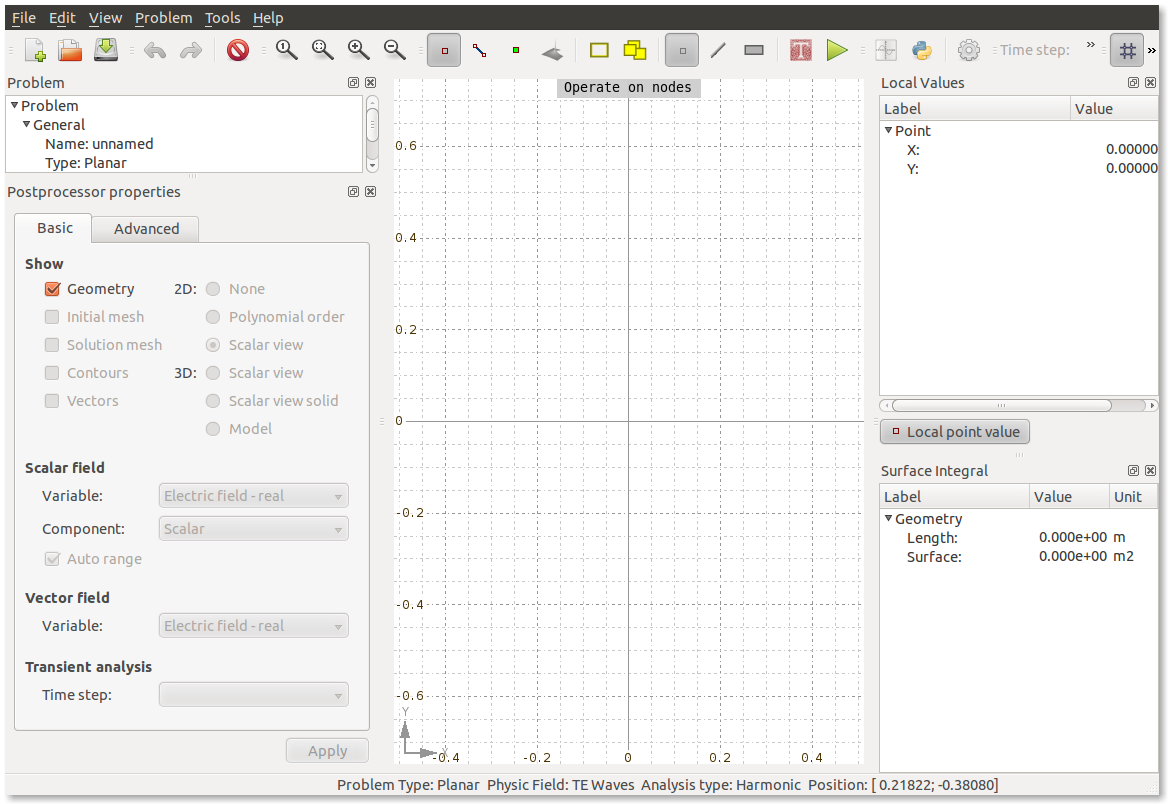
\includegraphics[width=14cm]{sim_agros2d.png}
	\caption{Základní pracovní rostředí programu Agros2D.}
	\label{obr:sim_agros2d}
\end{figure}

Samotný modul pro simulaci elektromagnetického pole tedy využívá z programu Agros2D zmíněný preprocesor pro zadávání dat a postprocesor pro zobrazení výsledků ve 2D a 3D zobrazení. Vlastní numerické řešení zajišťuje knihovna Hermes2D a programový kód je obsažen v modulu  označeném jako TE Waves. V této kapitole jsou popsány výpočetní části, které se týkají především řešení vlnových rovnic, specifikace okrajových podmínek a zadávání materiálových konstant prostředí. 

\section{Předpoklady simulace}
Vzhledem k široké problematice elektromagnetických vln je potřeba pro jejich modelování zavést některé zjednodušení. 
\begin{itemize}
\item {\bf Harmonická analýza} - první předpokladem je řešení vlnové rovnice v harmonickém tvaru (Helmholtzova rovnice)
\begin{displaymath}
	\nabla^{2}\vecfaz E +\faz k^{2}\vecfaz E = 0.
\end{displaymath}
\item {\bf Šíření vln v kartézské souřadnicové soustavě v jediném směru dle osy z} - tento předpoklad platí pro planární problém.
\item {\bf Šíření vln v polární souřadnicové soustavě má pouze tangenciální složku} - uvažujeme pro osově symetrický problém.
\end{itemize}

\section{Metoda konečných prvků}
Základem samotné knihovny Hermes2D je numerické řešení pomocí tzv. metody konečných prvků neboli FEM (Finite Element Method). Historie spadá do první poloviny 20. století, kdy byly základy FEM popsány v práci a Richarda Couranta (1943). Až v roce 1953 byly rovnice popsány v maticovém tvaru, což umožnilo řešení na počítačích a v té době se FEM využívala v leteckém průmyslu. K jejímu šiřšímu využití v dalších oborech však došlo až s nástupem modernější výpočetní techniky v průběhu 60. a 70. let. Například na problémy týkající se elektromagnetismu nebyla FEM použita dříve než v roce 1968. V současné době se však pomocí FEM výhodně řeší fyzikální problémy z oborů statiky, dynamiky, akustiky, tepla, elektromagnetického pole, proudění, elektrostatiky a z dalších vědeckých disciplín. 

Ačkoliv existují také jiné numerické metody řešení, například metoda konečných diferencí (FDM) nebo momentová metoda (MOM), které nejsou tak náročné na programovou implementaci, tak právě FEM je metodou nejvíce používanou. Důvodem je její všestrannost a výkonnost. Dalším aspektem je to, že programy vyvinuté pro konkrétní problémy mohou být snadno použity k řešení příkladů v naprosto jiném oboru po drobných nebo žádných změnách.

\subsection{Kroky řešení pomocí FEM}
Analýza jakéhokoliv problému prostřednictvím metody konečných prvků zahrnuje v podstatě čtyři kroky:
\begin{itemize}
\item {Diskretizace oblasti na konečný počet prvků}
\item {Vyjádření rovnic pro konkrétní prvek}
\item {Sestavení prvků v řešené oblasti}
\item {Řešení získaných rovnic}
\end{itemize}
Princip řešení a odvození rovnic vychází z \cite[kap. 6.2]{num} pro jednoduchost reprezentován na Laplaceově rovnici $\nabla^{2}V = 0$.

\subsection*{Diskretizace}
Prvním krokem, shodným pro libovolnou, numericky řešenou rovnici, je rozdělení nekonečného objemu řešené oblasti na konečný počet prvků, tak jak je to naznačeno na obrázku \ref{obr:sim_diskretizace}.
\begin{figure}[!h]
	\centering
	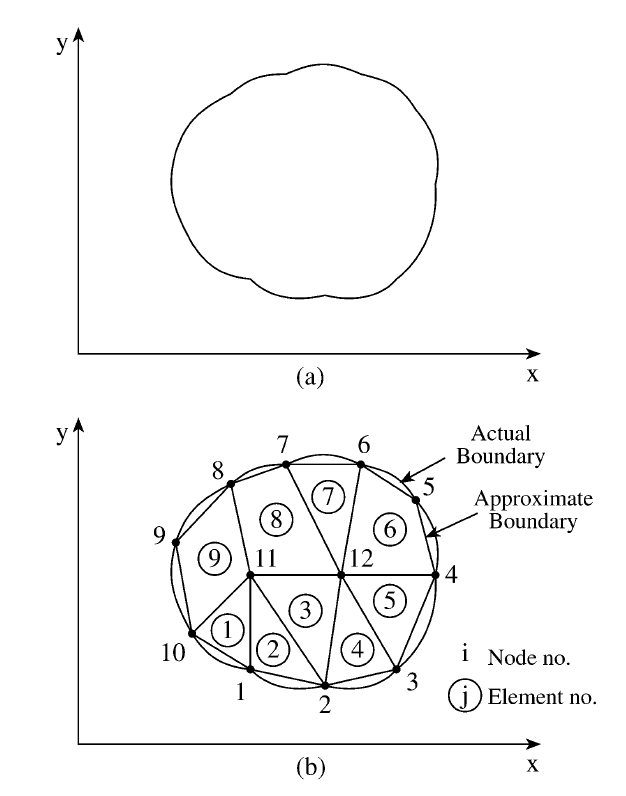
\includegraphics[width=8cm]{sim_diskretizace.png}
	\caption{Rozdělení řešené oblasti (a) na konečný počet diskretizačních prvků (b).\cite{num}}
	\label{obr:sim_diskretizace}
\end{figure}
Vlastní prvky, na které je oblast rozčleněna mohou mít libovolný tvar, ale typické tvary pro dvojdimenzionální problém jsou jsou naznačeny na obrázku \ref{obr:sim_prvky}.
\begin{figure}[!h]
	\centering
	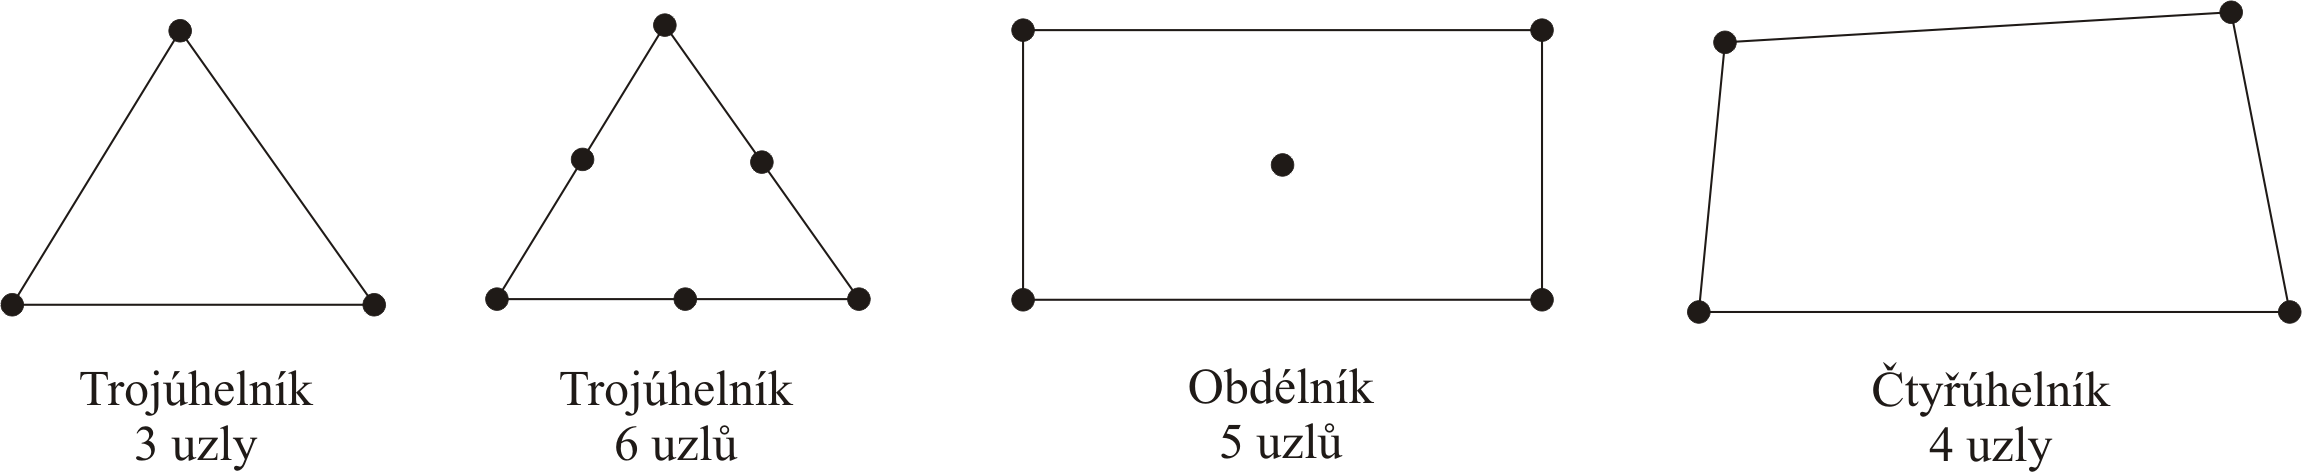
\includegraphics[width=9cm]{sim_prvky.png}
	\caption{Prvky diskterizace.\cite{num}}
	\label{obr:sim_prvky}
\end{figure}

\subsection*{Vyjádření rovnic pro aproximaci řešení}
V další části předpokládáme aproximaxi řešení na celé oblasti 
\begin{displaymath}
V(x,y) \simeq \sum_{e=1}^{N}V_e(x,y),
\end{displaymath}
kde N je počet prvků, do kterých je řešená oblast rozdělena. Aproximované řešení lze zapsat jako lineární kombinaci bázových funkcí s neznámými koeficienty, například $a$, $b$ a $c$
\begin{displaymath}
V_e(x,y) = a + bx + cy.
\end{displaymath}



\section{Řešení harmonické vlnové rovnice knihovnou Hermes2D} \label{sec:sim_hermes2d}
\subsection{Kartézská souřadná soustava} \label{subsec:sim_kar}
Po zavedení zjednodušujících předpokladů vycházíme z rovnice ve tvaru
\begin{equation}
	\nabla^{2}\faz E_{(z)} +\faz k^{2}\faz E_{(z)} = 0
	\label{rce:sim_kar_helmholtz_num} 
\end{equation}
platné na definované oblasti $\Omega$, na které známe okrajové podmínky a ve které chceme dostat výsledné řešení. Tím může být například vnitřní prostor vlnovodu nebo rezonátoru. Pro získání slabé formy k rovnici (\ref{rce:sim_kar_helmholtz_num}) nejprve vyjádříme reálnou a imaginární složku
\begin{displaymath}
	\nabla^{2}(E_R + \mj E_I) + (\omega^{2}\varepsilon\mu - \mj\omega\mu\sigma)(E_R + \mj E_I) = 0,
\end{displaymath}
\begin{displaymath}
	\nabla^{2} E_R + \mj\nabla^{2} E_I + \omega^{2}\varepsilon\mu E_R + \mj\omega^{2}\varepsilon\mu E_I - \mj\omega\mu\sigma E_R + \omega\mu\sigma E_I = 0,
\end{displaymath}
kde reálnou část tvoří
\begin{equation}
	\Re : \nabla^{2} E_R + \omega^{2}\varepsilon\mu E_R + \omega\mu\sigma E_I = 0,
	\label{rce:sim_kar_num_real} 
\end{equation}
a imaginární je vyjádřena
\begin{equation}
	\Im : \nabla^{2} E_I + \omega^{2}\varepsilon\mu E_I - \omega\mu\sigma E_R = 0.
	\label{rce:sim_kar_num_imag} 
\end{equation}
Obě upravené rovnice (\ref{rce:sim_kar_num_real}) a (\ref{rce:sim_kar_num_imag}) je již možné převést do slabých forem, které splňují nulovou Dirichletovu a Neumannovu okrajovou podmínku. Postup převodu spočívá ve vynásobení parciálních diferenciálních rovnic testovací funkcí $v$ a v následné integraci přes oblast řešení $\Omega$ 
\begin{equation}
	\Re : \int_{\Omega}\nabla^{2} E_R\cdot v \dif S + \omega^{2}\varepsilon\mu\int_{\Omega} E_R\cdot v\dif S + \omega\mu\sigma\int_{\Omega} E_I\cdot v\dif S = 0,
	\label{rce:sim_kar_weak_odv_real} 
\end{equation}
\begin{equation}
	\Im : \int_{\Omega}\nabla^{2} E_I\cdot v\dif S + \omega^{2}\varepsilon\mu\int_{\Omega} E_I\cdot v\dif S - \omega\mu\sigma\int_{\Omega} E_R\cdot v\dif S = 0.
	\label{rce:sim_kar_weak_odv_imag} 
\end{equation}
V dalším kroku se aplikuje 1. Greenova identita \cite[příloha A.2]{num} (integrace po částech pro vyšší řády) a tím se konečně získají slabé formy k původním rovnicím (\ref{rce:sim_kar_num_real}) a (\ref{rce:sim_kar_num_imag})
\begin{equation}
	\Re : \int_{\Gamma}\frac{\partial E_R}{\partial n}\cdot v\dif l-\int_{\Omega}\nabla E_R\cdot\nabla v \dif S + \omega^{2}\varepsilon\mu\int_{\Omega} E_R\cdot v\dif S + \omega\mu\sigma\int_{\Omega} E_I\cdot v\dif S = 0,
	\label{rce:sim_kar_weak_real} 
\end{equation}
\begin{equation}
	\Im : \int_{\Gamma}\frac{\partial E_I}{\partial n}\cdot v\dif l-\int_{\Omega}\nabla E_I\cdot\nabla v\dif S + \omega^{2}\varepsilon\mu\int_{\Omega} E_I\cdot v\dif S - \omega\mu\sigma\int_{\Omega} E_R\cdot v\dif S = 0.
	\label{rce:sim_kar_weak_imag} 
\end{equation}
První člen $\int_{\Gamma}\frac{\partial E_R}{\partial n}\cdot v\dif l$ (respektive $\int_{\Gamma}\frac{\partial E_I}{\partial n}\cdot v\dif l$) vyjadřuje Neumanovu okrajovou podmínku. Pokud je podmínka nulová, tak i tyto členy budou nulové. Levé strany rovnic (\ref{rce:sim_kar_weak_real}) a (\ref{rce:sim_kar_weak_imag}) představují bilineární členy daných slabých forem. Lineární členy jsou nulové, neboť se nacházejí na pravých stranách rovnic. 

\subsubsection*{Kód k řešení bilineární části rovnice (\ref{rce:sim_kar_weak_real})}
Pro zápis programového kódu vztahující se k rovnici (\ref{rce:sim_kar_weak_real}) rozdělíme bilineární část na složky reprezentované $E_{R}$ a $E_{I}$. První vyjádříme zápis, který je v programu označen indexem \uv{real\_real}. Rozepsáním operátoru $\nabla$ a numerickým řešením integrálů obdržíme výraz
\begin{equation}
	-\sum_{i=0}^{n}\mathrm{w}_{t}[i]\bigg(\frac{\partial E_R}{\partial x}\cdot \frac{\partial v}{\partial x} + \frac{\partial E_R}{\partial y}\cdot \frac{\partial v}{\partial y} \bigg) + \omega^{2}\varepsilon\mu\sum_{i=0}^{n}\mathrm{w}_{t}[i]\bigg(E_R\cdot v\bigg),
	\label{rce:sim_kar_weak_real_real_num} 
\end{equation}
Vlastní programový kód, který implemetuje bilineární část (\ref{rce:sim_kar_weak_real_real_num}), je následující

\begin{verbatim}
template<typename Real, typename Scalar>
Scalar rf_matrix_form_real_real(int n, double *wt, Func<Real> *u_ext[], Func<Real> *u,
                                    Func<Real> *v, Geom<Real> *e, ExtData<Scalar> *ext)
{
    return - int_grad_u_grad_v<Real, Scalar>(n, wt, u, v)
    + sqr(2 * M_PI * frequency) * (rfLabel[e->elem_marker].permeability * MU0)
    * (rfLabel[e->elem_marker].permittivity * EPS0) * int_u_v<Real, Scalar>(n, wt, u, v);
}
\end{verbatim}
Obdobným způsobem postupujeme u druhé složky bilineární části vyjádřené pomocí $E_I$. Index funkce v programu se změní na \uv{real\_imag}
\begin{equation}
 \omega\mu\sigma\sum_{i=0}^{n}\mathrm{w}_{t}[i]\bigg(E_I\cdot v\bigg)
	\label{rce:sim_kar_weak_real_imag_num} 
\end{equation}
Vztah \ref{rce:sim_kar_weak_real_imag_num} se analogicky zapíše jako
\begin{verbatim}
template<typename Real, typename Scalar>
Scalar rf_matrix_form_real_imag(int n, double *wt, Func<Real> *u_ext[], Func<Real> *u,
                                     Func<Real> *v, Geom<Real> *e, ExtData<Scalar> *ext)
{
    return + 2 * M_PI * frequency * (rfLabel[e->elem_marker].permeability * MU0) 
    * rfLabel[e->elem_marker].conductivity * int_u_v<Real, Scalar>(n, wt, u, v);
}
\end{verbatim}

\subsubsection*{Kód k řešení bilineární části rovnice (\ref{rce:sim_kar_weak_imag})}
Postup je naprosto totožný jako u slabé formy reálné složky výchozí rovnice. Tudíž opět rozdělíme bilineární část na 2 části dle $E_R$ a $E_I$. Dále zavedeme numerickou integraci a zapíšeme vzniklé výrazy do programového kódu. Pro index \uv{imag\_real} platí
\begin{equation}
 -\omega\mu\sigma\sum_{i=0}^{n}\mathrm{w}_{t}[i]\bigg(E_I\cdot v\bigg)
	\label{rce:sim_kar_weak_imag_real_num} 
\end{equation}
\begin{verbatim}
template<typename Real, typename Scalar>
Scalar rf_matrix_form_imag_real(int n, double *wt, Func<Real> *u_ext[], Func<Real> *u,
									Func<Real> *v, Geom<Real> *e, ExtData<Scalar> *ext)
{
    return - 2 * M_PI * frequency * (rfLabel[e->elem_marker].permeability * MU0) 
    * rfLabel[e->elem_marker].conductivity * int_u_v<Real, Scalar>(n, wt, u, v);
}
\end{verbatim}
Nakonec pro označení \uv{imag\_imag}
\begin{equation}
	-\sum_{i=0}^{n}\mathrm{w}_{t}[i]\bigg(\frac{\partial E_I}{\partial x}\cdot \frac{\partial v}{\partial x} + \frac{\partial E_I}{\partial y}\cdot \frac{\partial v}{\partial y} \bigg) + \omega^{2}\varepsilon\mu\sum_{i=0}^{n}\mathrm{w}_{t}[i]\bigg(E_I\cdot v\bigg),
	\label{rce:sim_kar_weak_imag_imag_num} 
\end{equation}
\begin{verbatim}
template<typename Real, typename Scalar>
Scalar rf_matrix_form_imag_imag(int n, double *wt, Func<Real> *u_ext[], Func<Real> *u,
                                    Func<Real> *v, Geom<Real> *e, ExtData<Scalar> *ext)
{
    return - int_grad_u_grad_v<Real, Scalar>(n, wt, u, v) 
    + sqr(2 * M_PI * frequency) * (rfLabel[e->elem_marker].permeability * MU0) 
    * (rfLabel[e->elem_marker].permittivity * EPS0) * int_u_v<Real, Scalar>(n, wt, u, v);
}
\end{verbatim}

\subsubsection*{Zápis lineárních členů rovnic (\ref{rce:sim_kar_weak_real}) a (\ref{rce:sim_kar_weak_imag}).}
Lineární členy jsou vyjádřeny jako pravé strany rovnic (\ref{rce:sim_kar_weak_real}) a (\ref{rce:sim_kar_weak_imag}). Jsou tudíž nulové, ale pro vlastní numerické řešení je potřeba tuto informaci doplnit do programového kódu. Vzhledem k tomu, že řešená rovnice je komplexního charakteru je potřeba doplnit tyto dvě funkce 

\begin{verbatim}
template<typename Real, typename Scalar>
Scalar rf_vector_form_real(int n, double *wt, Func<Real> *u_ext[], Func<Real> *v,
                                               Geom<Real> *e, ExtData<Scalar> *ext)
{
    return 0.0;
}
\end{verbatim}
\begin{verbatim}
template<typename Real, typename Scalar>
Scalar rf_vector_form_imag(int n, double *wt, Func<Real> *u_ext[], Func<Real> *v, 
                                              Geom<Real> *e, ExtData<Scalar> *ext)
{
    return 0.0;
}
\end{verbatim}
Zmíněné funkce pro řešení Helmholtzovy rovnice (\ref{rce:sim_kar_helmholtz_num}) je dále potřeba zaregistrovat ve třídě \textsc{WeakForm} následujícím způsobem
\begin{verbatim}
wf->add_matrix_form(0, 0, callback(rf_matrix_form_real_real));
wf->add_matrix_form(0, 1, callback(rf_matrix_form_real_imag));
wf->add_matrix_form(1, 0, callback(rf_matrix_form_imag_real));
wf->add_matrix_form(1, 1, callback(rf_matrix_form_imag_imag));
wf->add_vector_form(0, callback(rf_vector_form_real))
wf->add_vector_form(1, callback(rf_vector_form_imag));
\end{verbatim}

\subsection{Polární souřadná soustava}
Řešení vlnové rovnice v polárních souřadnicích vychází z rovnice
\begin{equation}
	\nabla\times(\nabla\times\vecfaz E) +\faz k^{2}\vecfaz E = 0.
	\label{rce:sim_pol_helmholtz_num} 
\end{equation}
Po zavedení zjednodušení, že výsledné řešení má pouze tangenciální složku, můžeme rovnici \ref{rce:sim_pol_helmholtz_num} snadno upravit. Nejprve vyjádříme vnitřní rotaci
\begin{displaymath}
	\nabla\times \frac{1}{r}\Bigg|
	\begin{array}{ccc}
\hat{r} & r\hat{\alpha} & \hat{z} \\
\frac{\partial}{\partial r} & \frac{\partial}{\partial \alpha} & \frac{\partial}{\partial z} \\
0 & r\faz E_{\alpha} & 0\\
\end{array}\Bigg| +\faz k^{2}\faz E_{\alpha} = 0,
\end{displaymath}
\begin{equation}
\nabla\times \Bigg[\hat{r}\bigg(-\frac{1}{r}\cdot\frac{\partial r\faz E_{\alpha}}{\partial z}\bigg) + \hat{\alpha}\bigg(0\bigg) + \hat{z}\bigg(\frac{1}{r}\cdot\frac{\partial r\faz E_{\alpha}}{\partial r}\bigg) \Bigg]+\faz k^{2}\faz E_{\alpha} = 0.
	\label{rce:sim_pol_rotace1}
\end{equation}
Analogickým způsobem upravíme vnější rotaci ve vztahu (\ref{rce:sim_pol_rotace1})
\begin{displaymath}
	\frac{1}{r}\Bigg|
	\begin{array}{ccc}
\hat{r} & r\hat{\alpha} & \hat{z} \\
\frac{\partial}{\partial r} & \frac{\partial}{\partial \alpha} & \frac{\partial}{\partial z} \\
-\frac{1}{r}\cdot\frac{\partial r\faz E_{\alpha}}{\partial z} & 0 & \frac{1}{r}\cdot\frac{\partial r\faz E_{\alpha}}{\partial r}\\
\end{array}\Bigg| +\faz k^{2}\faz E_{\alpha} = 0,
\end{displaymath}
\begin{equation}
\Bigg[\hat{r}\bigg(\frac{1}{r}\cdot\frac{\partial}{\partial \alpha}\cdot\frac{1}{r}\frac{\partial r\faz E_{\alpha}}{\partial r}\bigg) + \hat{\alpha}\bigg(-\frac{\partial}{\partial z}\cdot\frac{1}{r}\cdot\frac{\partial r\faz E_{\alpha}}{\partial z} - \frac{\partial}{\partial r}\cdot\frac{1}{r}\cdot\frac{\partial r\faz E_{\alpha}}{\partial r}\bigg) + \hat{z}\bigg(\frac{1}{r}\cdot\frac{\partial}{\partial \alpha}\cdot\frac{1}{r}\frac{\partial r E_{\alpha}}{\partial z}\bigg) \Bigg]+\faz k^{2}\faz E_{\alpha} = 0.
	\label{rce:sim_pol_rotace2}
\end{equation}
Ve výsledném vztahu (\ref{rce:sim_pol_rotace2}) zanedbáme všechny ostatní složky kromě té, která respektuje souřadnici $\hat{\alpha}$. Dostaneme rovnici
\begin{displaymath}
-\frac{\partial}{\partial z}\cdot\frac{1}{r}\cdot\frac{\partial r\faz E_{\alpha}}{\partial z} - \frac{\partial}{\partial r}\cdot\frac{1}{r}\cdot\frac{\partial r\faz E_{\alpha}}{\partial r}+\faz k^{2}\faz E_{\alpha} = 0,
\end{displaymath}
kterou upravíme do podoby
\begin{equation}
-\frac{\partial^{2}E_{\alpha}}{\partial z^{2}}-\frac{\partial^{2}E_{\alpha}}{\partial r^{2}}-\frac{1}{r}\cdot\frac{\partial E_{\alpha}}{\partial r} + \frac{E_{\alpha}}{r^{2}} +\faz k^{2}\faz E_{\alpha} = 0.
	\label{rce:sim_pol_helmholtz_upravena}
\end{equation}
Tento vztah představuje vyjádření Helmholtzovy rovnice v polárních souřadnicích, při uvažování výše uvedených předpokladů simulace. Pro zápis programového kódu k vyřešení rozložení pole při osové symetrii je potřeba, stejným způsobem jako v podkapitole \ref{subsec:sim_kar}, odvodit slabou formu k rovnici (\ref{rce:sim_pol_helmholtz_upravena}) 
splňující Dirichletovu i Neumannovu okrajovou podmínku. 

\subsubsection*{Numerické řešení rovnice (\ref{rce:sim_pol_helmholtz_upravena})}
Bilineární člen dané slabé formy s indexem \uv{real\_real} lze po zavedení numerické integrace zapsat jako
\begin{displaymath}
-\sum_{i=0}^{n}\mathrm{w}_{t}[i]\bigg(\frac{\partial E_{\alpha R}}{\partial z}\cdot \frac{\partial v}{\partial z} + \frac{\partial E_{\alpha R}}{\partial r}\cdot \frac{\partial v}{\partial r} \bigg) - \frac{1}{r}\sum_{i=0}^{n}\mathrm{w}_{t}[i]\bigg(\frac{\partial E_{\alpha R}}{\partial r}\cdot v\bigg) +
\end{displaymath}
\begin{equation}
	 + \frac{1}{r^{2}}\sum_{i=0}^{n}\mathrm{w}_{t}[i]\bigg(E_{\alpha R}\cdot v\bigg) + \omega^{2}\varepsilon\mu\sum_{i=0}^{n}\mathrm{w}_{t}[i]\bigg(E_{\alpha R}\cdot v\bigg).
	\label{rce:sim_pol_bilinear_real_real} 
\end{equation}
Je zřejmé, že forma označená \uv{real\_imag} vyjde identicky jako v případě kartézské souřadné soustavy, neboť člen $+\faz k^{2}\faz E_{\alpha}$ v rovnici (\ref{rce:sim_pol_helmholtz_upravena}) je formálně stejný se vztahem (\ref{rce:sim_kar_helmholtz_num}). Platí tedy
\begin{equation}
 \omega\mu\sigma\sum_{i=0}^{n}\mathrm{w}_{t}[i]\bigg(E_{\alpha I}\cdot v\bigg).
	\label{rce:sim_pol_bilinear_real_imag} 
\end{equation}
Slabým formám vycházející z imaginární části z původní rovnice (\ref{rce:sim_pol_helmholtz_upravena}) odpovídá vyjádření
\begin{equation}
 -\omega\mu\sigma\sum_{i=0}^{n}\mathrm{w}_{t}[i]\bigg(E_{\alpha R}\cdot v\bigg)
	\label{rce:sim_pol_bilinear_imag_imag} 
\end{equation}
pro \uv{imag\_real}, což je opět ze stejného důvodu identické s kartézskou souřadnou soustvou. Nakonec indexu \uv{imag\_imag} odpovídá
\begin{displaymath}
-\sum_{i=0}^{n}\mathrm{w}_{t}[i]\bigg(\frac{\partial E_{\alpha I}}{\partial z}\cdot \frac{\partial v}{\partial z} + \frac{\partial E_{\alpha I}}{\partial r}\cdot \frac{\partial v}{\partial r} \bigg) - \frac{1}{r}\sum_{i=0}^{n}\mathrm{w}_{t}[i]\bigg(\frac{\partial E_{\alpha I}}{\partial r}\cdot v\bigg) +
\end{displaymath}
\begin{equation}
	 + \frac{1}{r^{2}}\sum_{i=0}^{n}\mathrm{w}_{t}[i]\bigg(E_{\alpha I}\cdot v\bigg) + \omega^{2}\varepsilon\mu\sum_{i=0}^{n}\mathrm{w}_{t}[i]\bigg(E_{\alpha I}\cdot v\bigg).
	\label{rce:sim_pol_bilinear_real_real} 
\end{equation}
Vzhledem k nulové pravé straně řešené výchozí rovnice (\ref{rce:sim_pol_helmholtz_upravena}) bude lineární člen  v tomto případě opět nulový.

\subsection{Numerická integrace}
Výpočet určitých interálů, který se v řešených vztazích vyskytují, je analyticky možný pouze v určitých jednoduchých případech. Pro obecné funkce se integrace provádí numericky. Jednou z možností je výpočet pomocí Gaussovy kvadratury.

Účelem je vypočítat numericky hodnodutu integrálu obecné funkce $g(\xi)$ na intervalu $x\in\langle a, b\rangle$,  pomocí aproximace výrazem
\begin{displaymath}
\sum_{i=0}^{n}\mathrm{w}_{t}[i]f(x_{i}),
\end{displaymath}
který se nazývá kvadraturní formule. Číslo $n$ představuje počet integračních bodů, hodnoty $\mathrm{w}_{t}[i]$ jsou příslušné váhové koeficienty uvedeného kvadraturního vzorce a $x_{i}$ se nazývají jeho uzly. 

Při výpočtu integrálu pomocí kvadraturní formule záleží tedy na volbě dělících bodů $x_{i}$ i koeficientů $\mathrm{w}_{t}[i]$. Právě princip Gaussovy kvadratury spočívá v tom, jak vhodně zvolit $x_{i}$ a následně dopočítat $\mathrm{w}_{t}[i]$. Hodnoty uzlových bodů se pro jednorozměrný případ volí jako kořeny Legendrových polynomů
\begin{displaymath}
	P_{n}(x) = \frac{1}{2^{n}\cdot n!}\frac{\dif^{n}}{\dif x^{n}}[(x^{2} - 1)^{n}]
\end{displaymath}
a koeficienty $\mathrm{w}_{t}[i]$ jsou definovány
\begin{displaymath}
\mathrm{w}_{t}[i] = \frac{-2}{(n+2)P_{n+2}(x_i)P'_{n+1}(x_i)}
\end{displaymath}
Více o této metodě Gaussovy kvadratury je možné zjistit v \cite{gk_tichy} nebo v \cite{gk_kaw}.

\section{Okrajové podmínky}
Pro řešení diferenciálních rovnic popisující chování elektromagnetického pole v dané oblasti $\Omega$ je třeba znát okrajové podmínky na hranicích. Účelem je specifikovat chování výsledné funkce, případně derivace této funkce, v daných bodech ležících na okraji řešené oblasti. Při popisu fyzikálních polí pomocí diferenciálních rovnic se užívá Dirichletova, Neumannova nebo Newtonova (smíšená) okrajová podmínka.
\begin{itemize}
\item {\bf Dirichletova okrajová podmínka} - předepisuje na hranici $\Gamma$ hodnotu funkce $E_{(z)}$, která může být obecně závislá na čase nebo na souřadnicích
\begin{displaymath}
	E_{(z)}|_{\Gamma} = f_{Dir}(x,y,z,t). 
\end{displaymath}
\item {\bf Neumannova okrajová podmínka} - na okraji řešené oblasti definuje tato podmínka definuje hodnotu normálové derivace funkce $\frac{\partial E_{(z)}}{\partial n}$
\begin{displaymath}
	\frac{\partial E_{(z)}}{\partial n}|_{\Gamma} = f_{Neu}(x,y,z,t). 
\end{displaymath}
\item {\bf Newtonova okrajová podmínka} - neboli smíšená kombinuje obě předchozí uvedené okrajové podmínky. Na hranici $\Gamma$ tak specifikuje kombinaci hodnoty funkce $E_{(z)}$ a její normálové derivace $\frac{\partial E_{(z)}}{\partial n}$
\begin{displaymath}
	\bigg(\frac{\partial E_{(z)}}{\partial n} + E_{(z)}\bigg)|_{\Gamma} = f_{New}(x,y,z,t). 
\end{displaymath}
\end{itemize}

\subsection{Okrajové podmínky v simulačním modulu}
Při řešení problémů vztahující se k elektromagnetickému poli je možné použít na řešenou oblast několik typů okrajových podmínek, které se zadávají v dialogu \uv{new boundary condition}. Ten je možné zpřístupnit po pravém kliknutí na pracovní plochu a vybrání daného odkazu, případně je možné se na něj dostat klávesovou zkratkou Alt + B. Po zadání označení se vybere v rozbalovacím menu některá z definovaných okrajových podmínek.

\subsubsection*{Electric field}
První možností je zadat Dirichletovu podmínka na určité hranici $\Gamma$. Hodnotu okrajové podmínky zadáme jako komplexní číslo ve formátu reálné a imaginární složky, jak je znázorněno na obrázku \ref{obr:sim_BC_electric_field} pro číslo $0 + \mj 0$. Tato konkrétní okrajová podmínka se v oboru vysokofrekvenční techniky označuje jako \uv{perfect electric conductor}.
\begin{figure}[!h]
	\centering
	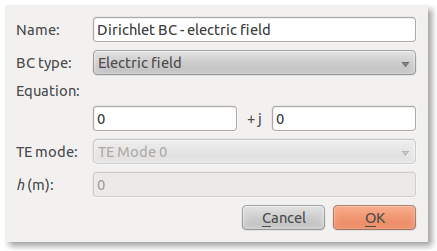
\includegraphics[width=7cm]{sim_BC_electric_field.png}
	\caption{Zadání Dirichletovy podmínky $0 + \mj 0$ pro elektrickou složku pole.}
	\label{obr:sim_BC_electric_field}
\end{figure}

Programový kód, který přísluší k této okrajové podmínce, je v modulu zapsán nastavením tříd \textsc{BCTypes} a \textsc{BCValues} následovně
\begin{verbatim}
BCTypes bcTypesReal, bcTypesImag;
bcTypesReal.add_bc_dirichlet(i+1);
bcTypesImag.add_bc_dirichlet(i+1);
                
BCValues bcValuesReal, bcValuesImag;
bcValuesReal.add_const(i+1, edgeRFMarker->value_real.number);
bcValuesImag.add_const(i+1, edgeRFMarker->value_imag.number);
\end{verbatim}

\subsubsection*{Magnetic field}
Touto volbou zadáváme hodnotu normálové derivace funkce $\frac{\partial E_{(z)}}{\partial n}$, jenž představuje Neumannovu okrajovou podmínku na hranici $\Gamma$. Opět má charakter komplexní veličiny, ve slabých formách vyjádřených v (\ref{rce:sim_kar_weak_real} ) a (\ref{rce:sim_kar_weak_imag}) podmínka představuje členy $\int_{\Gamma}\frac{\partial E_R}{\partial n}\cdot v\dif l$, případně $\int_{\Gamma}\frac{\partial E_I}{\partial n}\cdot v\dif l$. Příslušný kód je zapsán třídou \textsc{BCTypes}
\begin{verbatim}
BCTypes bcTypesReal, bcTypesImag;
bcTypesReal.add_bc_neumann(i+1);
bcTypesImag.add_bc_neumann(i+1);               
\end{verbatim}
a funkcí vracející povrchovou lineární formu Neumannovy okrajové podmínky. V případě nulové Neumannovy okrajové podmínky však lze danou funkci vynechat, tak jako v tomto případě.

\subsubsection*{Matched boundary}
Pokud chceme na určené hranici zvolit impedanční přizpůsobení, učiníme tak v dialogu pro výběr následující možností dle obrázku \ref{obr:sim_BC_matched_boundary}. 
\begin{figure}[!h]
	\centering
	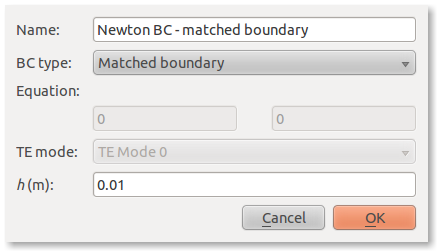
\includegraphics[width=7cm]{sim_BC_matched_boundary.png}
	\caption{Zadání impedančního přizpůsobení.}
	\label{obr:sim_BC_matched_boundary}
\end{figure}
Je zde možné zadat výšku hranice na kterou chceme aplikovat impedanční přizpůsobení pro výpočet konstatny $\beta$ ve vztahu (\ref{rce:sim_BC_matched_boundary}). V případě, že výšku nezadáme, bude výpočet impedančního přizpůsobení vycházet z vlnové impedance prostředí $Z = \frac{\omega\mu}{\beta}$. Ve výpočtu se tedy jedná se o Newtonovu okrajovou podmínku ve tvaru
\begin{equation}
	\bigg(\frac{\partial E_{(z)}}{\partial n} - \mj\beta E_{(z)}\bigg)|_{\Gamma} = 0.
	\label{rce:sim_BC_matched_boundary}
\end{equation}
Pro její implementaci je potřeba nastavit třídu \textsc{BCTypes} následovně
\begin{verbatim}
BCTypes bcTypesReal, bcTypesImag;
bcTypesReal.add_bc_newton(i+1);
bcTypesImag.add_bc_newton(i+1);              
\end{verbatim}
a také zapsat funkce pro povrchové bilineární formy. Pro reálnou složku odpovídá 
\begin{verbatim}
template<typename Real, typename Scalar>
Scalar rf_matrix_form_surf_imag_real(int n, double *wt, Func<Real> *u_ext[], Func<Real> *u,
                                         Func<Real> *v, Geom<Real> *e, ExtData<Scalar> *ext)
{
    if (!(rfEdge[e->edge_marker].type == PhysicFieldBC_RF_MatchedBoundary ||
          rfEdge[e->edge_marker].type == PhysicFieldBC_RF_Port))
    return 0.0;

    double mu = rfLabel[e->elem_marker].permeability * MU0;
    double eps = rfLabel[e->elem_marker].permittivity * EPS0;
    double height = rfEdge[e->edge_marker].height;
    double beta = 0.0;
    double Z = 0.0;

    if(!rfEdge[e->edge_marker].height == 0)
    {
        beta = sqrt(sqr(2 * M_PI * frequency) * mu * eps - sqr(1 * M_PI / height));
        return beta * int_u_v<Real, Scalar>(n, wt, u, v);
    }
    else
    {
        beta = sqrt(sqr(2 * M_PI * frequency) * mu * eps);
        Z = ((2 * M_PI * frequency) * mu ) / beta;
        return Z * int_u_v<Real, Scalar>(n, wt, u, v);
    }
}
\end{verbatim}
Pro imaginární část okrajové podmínky platí
\begin{verbatim}
template<typename Real, typename Scalar>
Scalar rf_matrix_form_surf_real_imag(int n, double *wt, Func<Real> *u_ext[], Func<Real> *u,
                                         Func<Real> *v, Geom<Real> *e, ExtData<Scalar> *ext)
{
    if (!(rfEdge[e->edge_marker].type == PhysicFieldBC_RF_MatchedBoundary ||
          rfEdge[e->edge_marker].type == PhysicFieldBC_RF_Port))
    return 0.0;

    double mu = rfLabel[e->elem_marker].permeability * MU0;
    double eps = rfLabel[e->elem_marker].permittivity * EPS0;
    double height = rfEdge[e->edge_marker].height;
    double beta = 0.0;
    double Z = 0.0;

    if(!rfEdge[e->edge_marker].height == 0)
    {
        beta = sqrt(sqr(2 * M_PI * frequency) * mu * eps - sqr(1 * M_PI / height));
        return beta * int_u_v<Real, Scalar>(n, wt, u, v);
    }
    else
    {
        beta = sqrt(sqr(2 * M_PI * frequency) * mu * eps);
        Z = ((2 * M_PI * frequency) * mu ) / beta;
        return Z * int_u_v<Real, Scalar>(n, wt, u, v);
    }
}
\end{verbatim}
Lineární část je u vztahu (\ref{rce:sim_BC_matched_boundary}) nulová, proto lze funkci pro její zápis vynechat.
Nakonec je potřeba výše uvedené funkce zaregistrovat ve třídě \textsc{WeakForm} takto
\begin{verbatim}
wf->add_vector_form_surf(0, callback(rf_vector_form_surf_real));
wf->add_vector_form_surf(1, callback(rf_vector_form_surf_imag));           
\end{verbatim}
                
\subsubsection*{Port}


\section{Vlastnosti prostředí}
V řešené rovnici (\ref{rce:sim_kar_helmholtz_num}) vystupují také materiálové konstatny prostředí, ve kterém se elektromagnetická vlna šíří. Pro jejich specifikaci je potřeba vytvořit materiál s těmito konstantami a vhodně jej přiřadit k příslušným značkám oblastí. Zpřístupnit dialog pro výběr lze opět pravým kliknutím na pracovní plochu a vybráním možnosti \uv{new material}, eventuelně zkratkou Alt + M. 
\begin{figure}[!h]
	\centering
	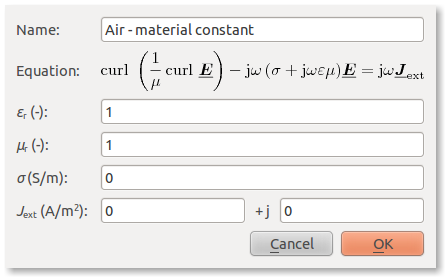
\includegraphics[width=7cm]{sim_material.png}
	\caption{Vytvoření materiálu vzduchu zadáním konstant prostředí.}
	\label{obr:sim_material}
\end{figure}
Parametry $\varepsilon_r$ a $\mu_r$ představují, tak jak je běžně používané, relativní hodnoty permitivity a permeability. Pomocí $\sigma$ zadáme vodivost v daném prostředí. Poslední parametr $J_{ext}$ představuje vnucený proud do oblasti, která je reprezentovaná danou značkou.

Programová implementace $J_{ext}$ spočívá v řešení Helmholtzovy rovnice (\ref{rce:sim_kar_helmholtz_num}) v případě nenulové pravé strany. Ta po převedení rovnice na slabou formu představuje její lineární část a je tak potřeba s ní nakládat. Vstupní rovnice pro implemetaci vnucené proudové hustoty je tedy
\begin{displaymath}
	\nabla^{2}\vecfaz E +\faz k^{2}\vecfaz E = \mathrm{grad}\frac{\rho}{\varepsilon} + \mj\omega\mu J_{ext}.
\end{displaymath}
Člen $\mathrm{grad}\frac{\rho}{\varepsilon}$ je možné zanedbat, vzhledem k předpokladu rovnoměrného rozložení náboje $\rho$. Při této úvaze bude hodnota gradientu nulová. Při převodu na slabou formu vyjádříme samostatně reálnou a imaginární složku vnější proudové husototy.
\begin{displaymath}
	\nabla^{2}(E_R + \mj E_I) + (\omega^{2}\varepsilon\mu - \mj\omega\mu\sigma)(E_R + \mj E_I) = \mj\omega\mu (J_{ext R} + \mj J_{ext I}). 
\end{displaymath}
Po rozdělení a převodu na slabé formy stejným způsobem jako v podkapitole \ref{sec:sim_hermes2d} dostaneme vztahy, ve kterých na pravé straně vystupují lineární členy 
\begin{equation}
	\Re : -\int_{\Omega}\nabla E_R\cdot\nabla v \dif S + \omega^{2}\varepsilon\mu\int_{\Omega} E_R\cdot v\dif S + \omega\mu\sigma\int_{\Omega} E_I\cdot v\dif S = -\omega\mu J_{ext I},
	\label{rce:sim_jext_real} 
\end{equation}
\begin{equation}
	\Im : -\int_{\Omega}\nabla E_I\cdot\nabla v\dif S + \omega^{2}\varepsilon\mu\int_{\Omega} E_I\cdot v\dif S - \omega\mu\sigma\int_{\Omega} E_R\cdot v\dif S = \omega\mu J_{ext R}.
	\label{rce:sim_jext_imag} 
\end{equation}
Programový kód pro řešení lineární části rovnic a je zapsán funkcemi, které vracející příslušnou lineární formu. Pro reálnou část v (\ref{rce:sim_jext_real}) je to
\begin{verbatim}
template<typename Real, typename Scalar>
Scalar rf_vector_form_real(int n, double *wt, Func<Real> *u_ext[], Func<Real> *v,
                                              Geom<Real> *e, ExtData<Scalar> *ext)
{
    Scalar result = 0 ;
    int u = 0;
    for (int i = 0; i < n; i++)
        result += wt[i] * (rfLabel[e->elem_marker].current_density_imag * v->val[i]);

    return - 2 * M_PI * frequency * (rfLabel[e->elem_marker].permeability * MU0) * result;
}
\end{verbatim}
a pro imaginární člen pravé strany v rovnici (\ref{rce:sim_jext_imag}) platí
\begin{verbatim}
template<typename Real, typename Scalar>
Scalar rf_vector_form_imag(int n, double *wt, Func<Real> *u_ext[], Func<Real> *v,
                                              Geom<Real> *e, ExtData<Scalar> *ext)
{
    Scalar result = 0 ;
    int u = 0;
    for (int i = 0; i < n; i++)
        result += wt[i] * (rfLabel[e->elem_marker].current_density_real * v->val[i]);

    return 2 * M_PI * frequency * (rfLabel[e->elem_marker].permeability * MU0) * result;
}
\end{verbatim}

\section{Typický postup řešení úloh v aplikaci Agros2D} 
Analýza fyzikálního pole ve všech programech zabývajících se touto problematikou bývá zpravidla rozdělena do třech základních etap. Toto obecné rozdělení je aplikované i v programu Agros2D.
\begin{itemize}
\item {\bf PreProcessing} - Prvním krokem je vytvoření modelu a definování jeho geometrických rozměrů. Dále je potřeba zvolit materiálové vlastnosti, nastavit parametry generování diskretizační sítě a typ analýzy.
\item {\bf Solution} - V další části probíhá vlastní řešení požadovaným řešičem.
\item {\bf PostProcessing} - Nakonec se provádí vyhodnocení řešeného problému.
\end{itemize}
Následující postup podrobněji rozepisuje kroky, které vedou k řešení konkrétních fyzikálních problémů.
\begin{enumerate}
\item Vytvoření a nastavení nového problému - volba řešeného fyzikálního pole, typu problému, druhu analýzy, zapnutí $h$, $p$ nebo $hp$ adaptivity, parametrů diskretizační sítě a frekvence
\begin{figure}[!h]
	\centering
	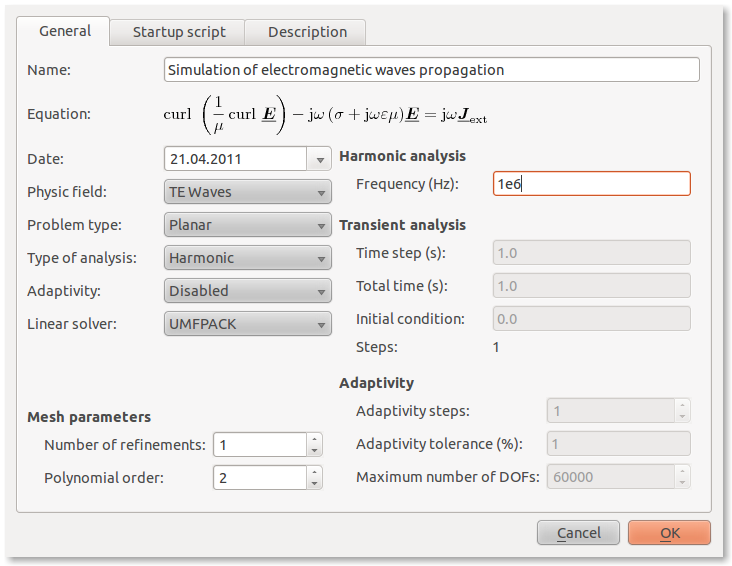
\includegraphics[width=9cm]{sim_problem_properties.png}
	\caption{Dialog vlastností problému programu Agros2d.}
	\label{obr:sim_problem_properties}
\end{figure}
\item Nakreslení struktury - pomocí vložení uzlů, zakreslení hranic mezi nimi a specifikování značek oblastí
\begin{itemize}
\item Nový uzel: po výběru nástroje \uv{operation on nodes} je možné vložit uzel přidržením Ctrl a levým kliknutém myši (případně pomocí dialogu vyvolaném stisknutím Alt + N)
\item Nová hrana: nástrojem \uv{operation on edges} se hranice vytvoří opět držením Ctrl a kliknutím mezi dva již vytvořené uzly (další možnost je kombinace Alt + E)
\item Nová značka oblastí: tu lze zadat nástrojem \uv{operation on labels} po držení Ctrl a kliku na požadované místo (Alt + L)
\end{itemize}
\item Vytvoření a bližší specifikace okrajových podmínek v dialogu \uv{new boundary condition} (klávesová zkratka Alt + B)
\item Přiřazení vytvořených podmínek na příslušnou hranu - to je možné po dvojkliku na hranu nebo kliknutím vybrat více hran a po stisku mezerníku zadat podmínku hromadně
\item Vytvoření materiálů a nastavení jejich parametrů v dialogu \uv{new material} (Alt + M)
\item Přiřazení vytvořených značek k dané ohraničené oblasti - lze také po dvojkliku na značku oblastí případně je to možné kombinací výběru myší a mezerníku
\item Diskretizace oblasti - globální úroveň lze nastavit při specifikaci problému, lokální nastavení lze provést u vlastností hrany nebo u značky oblasti 
\item Spuštění řešení
\begin{figure}[!h]
	\centering
	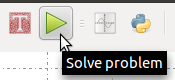
\includegraphics[width=3cm]{sim_spusteni_reseni.png}
\end{figure}
\item Volba vhodného zobrazení výsledků pomocí vlastností postprocesoru
\end{enumerate}

\section{Zobrazení výsledků řešení elektromagnetického pole}


 